\documentclass[11pt,a4paper]{article}
\usepackage{polski}
\usepackage[utf8]{inputenc}
\usepackage{amsthm}
\usepackage{graphicx}
\usepackage{hyperref} 
\usepackage{amsmath,amssymb}
\usepackage{float}

\newtheorem{defn}{Definicja}


\title{Metody iteracyjne Halleya i quasi-Halleya do rozwiązywania równań nieliniowych}
\author{Kamil Michalak}
\date{Analiza Numeryczna (M) - Zadanie P2.2}


\begin{document}
    \maketitle

    \section{Wstęp}
    \subsection{Opis zadania}
    Zadanie polega na rozpatrzeniu dwóch metod iteracyjnych, słuzących do rozwiązywania równań nieliniowych.\\\\
    Metody Halleya:
    $$
        x_{k+1} = x_k - \frac{f(x_k)}{f'(x_k)-\frac{f''(x_k)}{2f'(x_k)}f(x_k)},
    $$
    oraz metody quasi-Halleya:
    $$
        x_{k+1} = x_k - \frac{f(x_k)}{f'(x_k)-\frac{f'(x_k)-f'(x_{k-1})}{2(x_k-x_{k-1})f'(x_k)}f(x_k)}.
    $$

    Należy wyprowadzić powyższe wzory korzystając ze wzoru na metodę Newtona, a także obliczyć rzędy zbieżności tych metod. Następnie wybrać kilka przykładowych funkcji i porównać obie metody w praktyce.
    \subsection{Dane techniczne}
    Wszystkie programy wykorzystywane w eksperymentach zaprogramowałem w języku Julia, w wersji 1.0.1. Do obliczeń wykorzystywałem liczby zmiennoprzecinkowe o precyzji 1024 (1024 bity na mantysę). Obliczenia przeprowadziłem na komputerze z procesorem Intel Core i5 i 8 GB pamięci RAM.
    \section{Wyprowadzenie wzorów}
    \subsection{Metoda Halleya}
    Wzór na metodę Halleya wynika z rozwinięcia funkcji w szereg Taylora (z dokładnością do drugiego wyrazu).
    $$
        f(x) \approx f(x_n) + f'(x_n)(x-x_n) + \frac{f''(x_n)}{2}(x-x_n)^2
    $$
    Gdzie $x_n$ jest przybliżonym rozwiązaniem równania $f(x) = 0$. Celem jest znalezienie punktu $x_{n+1}$ który jest rozwiązaniem równania
    $$
        0 = f(x_n) + f'(x_n)(x_{n+1}-x_n) + \frac{f''(x_n)}{2}(x_{n+1}-x_n)^2
    $$

    Wyciągając $(x_{n+1}-x_n)$ przed nawias z dwóch ostatnich składników Otrzymujemy

    $$
        0 = f(x_n) + (x_{n+1}-x_n)\left(f'(x_n)+\frac{f''(x_n)}{2}(x_{n+1}-x_n)\right)
    $$

    Z czego wynika

    $$
        x_{n+1} - x_n = -\left(f'(x_n)+\frac{f''(x_n)}{2}(x_{n+1}-x_n)\right)
    $$

    $$
        x_{k+1} = x_k - \frac{f(x_k)}{f'(x_k) - \frac{f''(x_k)}{2f'(x_k)}f(x_k)}
    $$

    Uzyskaliśmy wzór na metodę Halleya.

    Wzór ten możemy również uzyskać ze wzoru na metodę Newtona:
    $$
        x_{k+1}= x_k - \frac{g(x)}{g'(x)}
    $$
    podstawiając $g(x) = \frac{f(x)}{\sqrt{f'(x)}}$.\\
    Policzmy $g'(x)$.
    $$
        g'(x) = \left(\frac{f(x)}{\sqrt{f'(x)}}\right)' = \frac{f'(x)*f'(x) - f(x)*\frac{1}{2\sqrt{f'(x)}}*f''(x)}{[f'(x)]^2} = \frac{[f'(x)]^2-\frac{1}{2}f(x)f''(x)}{f'(x)\sqrt{f'(x)}}
    $$
    Podstawiając powyższe wzory do wzoru na metodę Newtona uzyskujemy:
    $$
        x_{k+1} = x_k - \frac{\frac{f(x_k)}{\sqrt{f'(x_k)}}}{\frac{[f'(x_k)]^2 - \frac{1}{2}f(x_k)f''(x_k)}{f'(x_k)\sqrt{f'(x_k)}}}
    $$
    $$
        x_{k+1} = x_k - \frac{f(x_k)}{\sqrt{f'(x_k)}} * \frac{f'(x_k)\sqrt{f'(x_k)}}{[f'(x_k)]^2 - \frac{1}{2}f(x_k)f''(x_k)}
    $$
    $$
        x_{k+1} = x_k - \frac{f(x_k)f'(x_k)}{[f'(x_k)]^2 - \frac{1}{2}f(x_k)f''(x_k)}
    $$
    $$
        x_{k+1} = x_k - \frac{f(x_k)}{f'(x_k) - \frac{f''(x_k)}{2f'(x_k)}f(x_k)}
    $$

    \subsection{Metoda quasi-Halleya}
    Wyprowadzenie wzoru na metodę quasi-Halley ze wzoru na metodę Halleya jest bardzo podobne do wyprowadzenia wzoru na metodę siecznych ze wzoru na metodę Newtona. Aby uzyskać wzór na metodę siecznych zastępujemy $f'(x_k)$ w metodzie Newtona ilorazem różnicowym.
    $$
        \frac{f(x_k) - f(x_{k-1})}{x_k - x_{k-1}}
    $$
    Uzyskujemy w ten sposób metodę siecznych.
    $$
        x_{k+1} = x_k - f(x_k)\frac{x_k - x_{k-1}}{f(x_k) - f(x_{k-1})}
    $$

    Żeby uzyskać wzór na metodę quasi-Halleya zastępujemy $f''(x_k)$ w metodzie Halleya ilorazem różnicowym $f'$:
    $$
        \frac{f'(x_k) - f'(x_{k-1})}{x_k - x_{k-1}}
    $$

    Otrzymujemy:

    $$
        x_{k+1}  = x_k - \frac{f(x_k)}{f'(x_k) - \frac{f'(x_k) - f'(x_{k-1})}{2(x_k - x_{k-1})f'(x_k)}f(x_k)}
    $$

    \section{Rzędy zbieżności metod}

    \begin{defn}
        Niech ciąg $a_k$ będzie zbieżny do $g$. Jeśli istnieją takie liczby rzeczywiste $p$ i $C$ $(C > 0)$, że
        $$
            \lim_{n \to \infty} \frac{|a_{n+1} - g|}{|a_n - q|^p} = C
        $$

        to $p$ nazywamy \textbf{wykładnikiem zbieżności} ciągu, a $C$ – \textbf{stałą asymptotyczną błędu}. Dla $p = 1$ oraz $0 < C < 1$ zbieżność jest \textbf{liniowa}, dla $p = 2$ – \textbf{kwadratowa}, dla $p = 3$ – \textbf{sześcienna}
    \end{defn}

    \subsection{Metoda Halleya}
    Metoda Halley ma zbieżność sześcienną, dowód jest następujący.\\

    Weźmy dowolną funkcję f. Załóżmy, że $f(g)=0$, ale $f'(g) \neq 0$ oraz, że metoda Halleya jest zbieżna do $g$ dla pewnego punktu początkowego $x_0$. Załóżmy też, że trzecia pochodna f istnieje i jest ciągła w pewnym otoczeniu $g$ i, że $x_n$ znajduje się w tym otoczeniu. Wtedy ze wzoru Taylora mamy:
    $$
        0 = f(g) = f(x_n) + f'(x_n)(g-x_n) + \frac{f''(x_n)}{2}(g-x_n)^2 + \frac{f'''(\xi)}{6}(g-x_n)^3
    $$
    oraz
    $$
        0 = f(g) = f(x_n) + f'(x_n)(g-x_n) + \frac{f''(\eta)}{2}(g-x_n)^2
    $$
    Gdzie $\xi$ i $\eta$ są liczbami spomiędzy $a$ i $x_n$. Mnożąc pierwsze równanie przez $2f'(x_n)$ i odejmując drugie równanie pomnożone przez $f''(x_n)(a-x_n)$ otrzymujemy:

    \begin{multline*}
        0 = 2f(x_n)f'(x_n) + 2[f'(x_n)]^2(g-x_n) + f'(x_n)f''(x_n)(g-x_n)^2 + \frac{f'(x_n)f'''(\xi)}{3}(g-x_n)^3\\
     - f(x_n)f''(x_n)(g-x_n) - f'(x_n)f''(x_n)(g-x_n)^2 - \frac{f'(x_n)f''(\eta)}{2}(g-x_n)^3
    \end{multline*}

    $$
        0 = 2f(x_n)f'(x_n) + \left(2[f'(x_n)]^2 - f(x_n)f''(x_n)\right)(g-x_n) + \left(\frac{f'(x_n)f'''(\xi)}{3} - \frac{f''(x_n)f''(\eta)}{2} \right)(g-x_n)^3
    $$

    Przerzucamy drugi składnik na lewą stronę i dzielimy przez\\ $2[f'(x_n)]^2 - f(x_n)f''(x_n)$, otrzymujemy:

    $$
        g - x_n = \frac{-2f(x_n)f'(x_n)}{2[f'(x_n)]^2-f(x_n)f''(x_n)} - \frac{2f'(x_n)f'''(\xi)-3f''(x_n)f''(\eta)}{6(2[f'(x_n)]^2 - f(x_n)f''(x_n))}(g-x_n)^3
    $$

    Z czego wynika:

    $$
        g - x_{n+1} = - \frac{2f'(x_n)f'''(\xi)-3f''(x_n)f''(\eta)}{12[f'(x_n)]^2-6f(x_n)f''(x_n)}(g-x_n)^3
    $$

    $$
        \frac{|x_{n+1} - g|}{|x_n-g|^3} =  \left|\frac{2f'(x_n)f'''(\xi)-3f''(x_n)f''(\eta)}{12[f'(x_n)]^2-6f(x_n)f''(x_n)}\right|
    $$

    Licząc granicę przy $n \to \infty$ ($x_n \to g$) otrzymujemy:

    $$
        \lim_{n \to \infty} \frac{|x_{n+1} - g|}{|x_n-g|^3} = \left|\frac{2f'(g)f'''(g)-3f'(g)f''(g)}{12[f'(g)]^2} \right| = C
    $$

    Co kończy dowód.

    Metoda Halleya jest więc lepsza od metody Newtona, która ma zbieżność kwadratową.

    \subsection{Metoda quasi-Halleya}
    Metoda quasi-Halleya ma wykładnik zbieżności $1+\sqrt{2} \leq p \leq 3$. Dowód w \href{http://benisrael.net/HALLEY-AMS.pdf}{[1]} (twierdzenie 3, str. 8).

    \section{Implementacja metod w Julii}

    Implementacja metod Halleya i quasi-Halleya wygląda następująco.


    \begin{verbatim}
        halley(f,f',f'',n,x0)
            x := x0
            for i = 0,1,...,n
                x := x - f(x) / (f'(x) - f''(x)/(2*f'(x)) * f(x))
            return x
    \end{verbatim}

    \begin{verbatim}
        quasi_halley(f,f',n,x0,x1)
            for i = 0,1,...,n
                x2 := x1 - f(x1) / (f'(x1)-
                    (f'(x1)-f'(x0))/2*(x1-x0)*f'(x1)*f(x1))
                x0 := x1
                x1 := x2
            return x2
    \end{verbatim}

    Zaimplementujmy również metody Newtona i siecznych w celach porównawczych.

    \begin{verbatim}
        newton(f,f',n,x0)
            x := x0
            for i = 0,1,...,n
                x = x - f(x)/f'(x)
            return x
    \end{verbatim}

    \begin{verbatim}
        secant(f,n,x0,x1)
            for i = 1,2,...,n
                x2 := x1 - f(x1)*(f(x1)-f(x0))/(x1-x0)
                x0 := x1
                x1 := x2
            return x2
    \end{verbatim}

    \section{Testy}

    W testach użyłem funkcji, których pierwiastki można obliczyć korzystając z funkcji bibliotecznych w języku Julia. W tabelach podałem liczbę dokładnych cyfr po przecinku uzyskanego wyniku, obliczoną ze wzoru:
    $$
        n = \lfloor-\log_{10}{\Delta x}\rfloor
    $$

    gdzie $$ \Delta x = \left|\frac{\bar{x}-x}{x}\right| $$
    jest błędem względnym uzyskanego wyniku.


    \subsection{Funkcja $f(x)=x^2-2$}

    Dokładny pierwiastek obliczony za pomocą  \verb!sqrt(BigFloat(2.0))!
    
    Porównanie metody Halleya i Newtona, $x_0 = 1.0$\\

    \begin{tabular}{|l|l|l|}
        \hline
        \textbf{k} & \textbf{Metoda Halleya} & \textbf{Metoda Newtona} \\
        \hline
        1 & 1 & 1 \\
        2 & 6 & 2 \\
        3 & 20 & 5 \\
        4 & 61 & 11 \\ 
        5 & 185 & 24 \\ 
        6 & 308 & 48 \\
        7 & 308 & 97 \\
        8 & 308 & 195 \\
        9 & 308 & 308 \\
        10 & 308 & 308 \\
        11 & 308 & 308 \\
        12 & 308 & 308 \\
        13 & 308 & 308 \\
        14 & 308 & 308 \\
        15 & 308 & 308 \\
        \hline
    \end{tabular}\\\\
    \newpage
    Porównanie metody quasi-Halleya i siecznych, $x_0 = 1.0$, $x_1 = 3.0$\\

    \begin{tabular}{|l|l|l|}
        \hline
        \textbf{k} & \textbf{Metoda quasi-Halleya} & \textbf{Metoda siecznych} \\
        \hline
        1 & 1 & 0 \\ 
        2 & 3 & 1 \\ 
        3 & 11 & 2 \\ 
        4 & 35 & 4 \\ 
        5 & 107 & 7 \\ 
        6 & 308 & 11 \\ 
        7 & 308 & 18 \\ 
        8 & 308 & 30 \\ 
        9 & 308 & 50 \\ 
        10 & 308 & 81 \\ 
        11 & 308 & 131 \\ 
        12 & 308 & 213 \\ 
        13 & 308 & 308 \\ 
        14 & 308 & 308 \\ 
        15 & 308 & 308 \\ 
        \hline
    \end{tabular}\\
    \begin{figure}[H]
        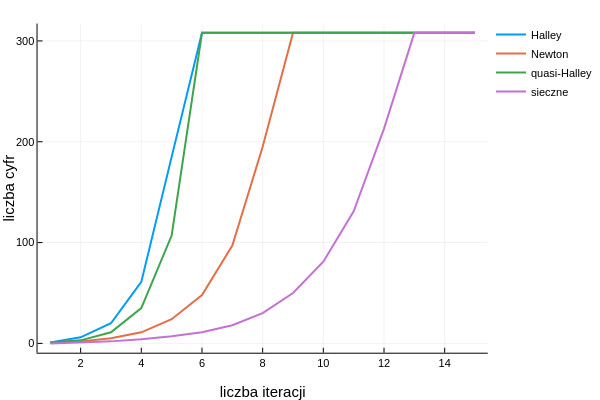
\includegraphics[width=0.9\textwidth]{wykr1}
        \caption{Wykres dokładności metod iteracyjnych dla funkcji $f(x) = x^2 - 2$}
    \end{figure}

    \subsection{Funkcja $\sin{x}$}

    $\pi$ jest miejscem zerowym funkcji, można więc użyć wbudowanej stałej \verb!pi! do sprawdzenia dokładności.\\
    
    $x_0 = 2.0$, $x_1 = 4.0$\\

    

    \begin{figure}[H]
        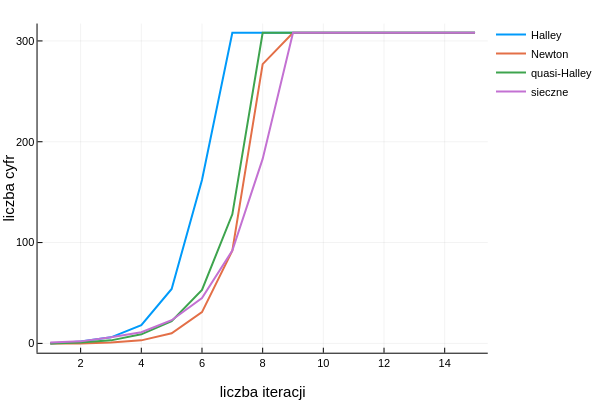
\includegraphics[width=0.9\textwidth]{wykr2}
        \caption{Wykres dokładności metod iteracyjnych dla funkcji $\sin{x}$}
    \end{figure}

    \subsection{Funkcja $f(x)=x^3-8$}

   
    $x_0 = 1.0, x_1 = 3.0$

    
    \begin{figure}[H]
        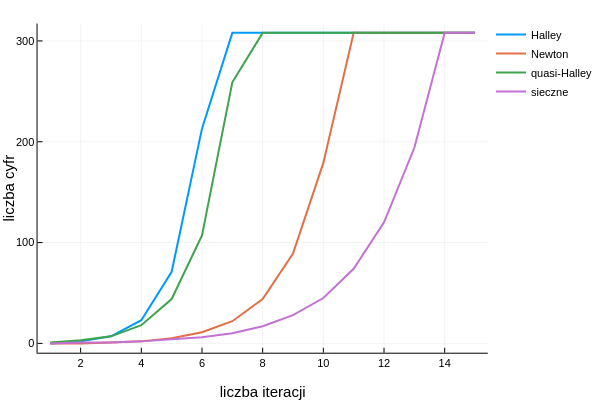
\includegraphics[width=0.9\textwidth]{wykr3}
        \caption{Wykres dokładności metod iteracyjnych dla funkcji $f(x)=x^3-8$}
    \end{figure}


    \subsection{Funkcja $f(x)=\sqrt{x}-3$}

    \begin{figure}[H]
        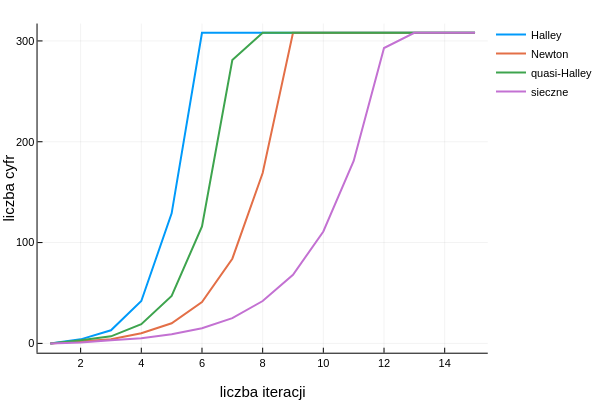
\includegraphics[width=0.9\textwidth]{wykr4}
        \caption{Wykres dokładności metod iteracyjnych dla funkcji $f(x)=\sqrt{x}-3$}
    \end{figure}



    \section{Wnioski}
    Metody iteracyjne Halleya i quasi-Halleya to metody iteracyjne pozwalające szybko znajdować pierwiastki funkcji. Mają lepszą zbieżność od metod Newtona i siecznych, co udowodniłem i sprawdziłem doświadczalnie. Są również proste w implementacji. Jedyną ich wadą w porówaniu z metodami Newtona i siecznych jest to, że wymagają policzenia większej ilości pochodnych, co w pewnych przypadkach może stanowić problem. Warto je stosować do funkcji, których pierwsza i druga pochodna nie jest bardzo trudna do policzenia.


    \section{Źródła}
    \begin{enumerate}
        \item \href{http://benisrael.net/HALLEY-AMS.pdf}{A. Ben-Israel, "Newton’s Method with Modified Functions", Contemporary Mathematics 204 (1997), 39–50.}
        \item \href{http://webdoc.sub.gwdg.de/ebook/dissts/Dortmund/Elhasadi2007.pdf}{Omar Ismael Elhasadi "Newton’s and Halley’s methods for real
        polynomials" }
    \end{enumerate}

\end{document}
